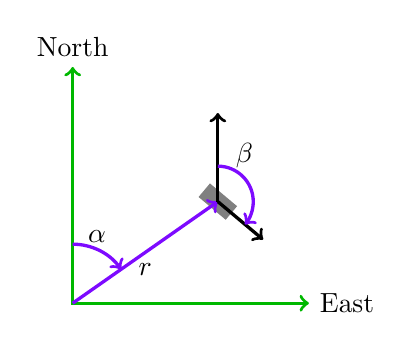
\begin{tikzpicture}[scale=1.5,line width=1.2pt]

  \definecolor{enu}{RGB}{0,184,0} % green
  \definecolor{compass}{RGB}{125,10,255} % purple
  \definecolor{base}{RGB}{128,128,128} % grey

  % Origin
  \coordinate (o) at (0,0);

  % Draw ENU axes
  \draw [enu,<->]
      (0,2) node[black] (yaxis) [above] {North} |-
      (2,0) node[black] (xaxis) [right] {East};

  % Draw a detectors
  \coordinate (d0) at (35:1.5);
  \fill[base,rotate=-40] (d0) ++(-.15,-.075) rectangle +(.3,.15);

  % Draw distance line
  \draw[compass,->] (o) -- node[black,below] {$r$} (d0);
  % Draw angle line
  \draw[compass,->] (0,.5) arc (90:35:.5);
  \draw[compass] (70:.6) node[black] {$\alpha$};

  % Draw North from detector
  \draw[->] (d0) -- +(0,.75);
  % Draw detector angle
  \draw[->] (d0) -- +(-40:.5);

  % Draw angle line
  \draw[compass,->] (d0) ++(0,.3) arc (90:-40:.3);
  \draw[compass] (d0) ++(60:.45) node[black] {$\beta$};

\end{tikzpicture}
